\documentclass{article}
\usepackage[top=0.75in, bottom=0.75in, left=1.25in, right=1in]{geometry} %formatage%
\usepackage{amsmath} %pour utiliser des maths de base%
\usepackage{amssymb} %pour faire \mathcal{}=>des lettres ''cursives''%
\usepackage{amsthm} % La petite boîte de fin de preuve
\usepackage{graphicx} %pour importer des images...http://www.tex.ac.uk/cgi-bin/texfaq2html?label=figurehere%
\usepackage{titlesec} %automatique, pour faire des sous-titres moins laids%
%\usepackage{cancel}
\usepackage[procnames]{listings}
\usepackage[utf8]{inputenc} 
\usepackage[T1]{fontenc}        %http://tex.stackexchange.com/questions/11897/draw-a-diagonal-arrow-across-an-expression-in-a-formula-to-show-that-it-vanishes%
\usepackage[frenchb]{babel}
\usepackage{xcolor}
\usepackage[squaren]{SIunits}
\usepackage{subcaption} % Avoir plusieurs sous-figures (graphiques) dans une figures et pouvoire les étiqueter
\usepackage{color}
\usepackage{lipsum}
\usepackage{caption}
\usepackage{wasysym}
\usepackage{braket}
\usepackage{mathtools}
\usepackage{mathrsfs} % Faire le symbole de la transformée de Laplace
\usepackage{bbm}
\usepackage{array}
\usepackage{diagbox}        
\usepackage{dsfont} % Faire des belles indicatrices                         %diagonale dans les tableaux
\usepackage{float}%placer les tableaux et images où tu veux
\usepackage{listings}
\usepackage[utf8]{inputenc}
\usepackage{comment}
\usepackage{pst-node}
\usepackage{fancyvrb} % Les varbatims gardent l'indentation
\usepackage{enumitem}
\usepackage{breakcites} % Faire en sorte que les citations ne sortent pas dans la marge
\usepackage{graphicx} % Insérer des graphiques
\usepackage{pgfplots}
\pgfplotsset{width=10cm, compat=1.9}
\usetikzlibrary{patterns,decorations.pathreplacing}

\newcommand{\tikzmark}[2]{%
	\tikz[remember picture,baseline=(#1.base)]
	\node[circle,red,draw,text=black,anchor=center,inner sep=1pt] (#1) {#2};}
\newcommand{\tikzmarkk}[2]{%
	\tikz[remember picture,baseline=(#1.base)]
	\node (#1) {#2};}


%\setcounter{secnumdepth}{0} % sections are level 1

\newtheorem{lemme}{Lemme}
\newtheorem{preuve}{Preuve}
\newtheorem{code}{Code informatique}
\newtheorem{exemple}{Exemple}
\newtheorem{scenario}{Scénario}

\begin{document}
	\renewcommand{\tablename}{Tableau}
	\renewcommand{\figurename}{Illustration}
	
	\begin{titlepage}
		\centering % Centre everything on the title page
		
		\scshape % Use small caps for all text on the title page
		
		\vspace*{7\baselineskip} % White space at the top of the page
		
		%------------------------------------------------
		%	Title
		%------------------------------------------------
		
		\rule{\textwidth}{1.6pt}\vspace*{-\baselineskip}\vspace*{2pt} % Thick horizontal rule
		\rule{\textwidth}{0.4pt} % Thin horizontal rule
		
		\vspace{0.75\baselineskip} % Whitespace above the title
		{\LARGE Calcul du tau de Kendall avec une variable aléatoire discrète et une continue. \\} % Title
		\vspace{0.75\baselineskip} % Whitespace below the title
		
		\rule{\textwidth}{0.4pt}\vspace*{-\baselineskip}\vspace{3.2pt} % Thin horizontal rule
		\rule{\textwidth}{1.6pt} % Thick horizontal rule
		
		\vspace{3\baselineskip} % Whitespace after the title block
		
		%------------------------------------------------
		%	Subtitle
		%------------------------------------------------
		{\scshape\Large Sous la supervision de \\Étienne Marceau\\} % Editor list
		
		\vspace*{3\baselineskip}
		
		  % Subtitle or further description
		
		\vspace*{3\baselineskip} % Whitespace under the subtitle
		
		%------------------------------------------------
		%	Editor(s)
		%------------------------------------------------
		
		Préparé par
		
		\vspace{0.5\baselineskip} % Whitespace before the editors
		
		{\scshape\Large Alexandre Lepage, \\
			Diamilatou N'diaye, \\} % Editor list
		
		\vspace*{5\baselineskip}
		
		le 18 juin 2019
		
		\vspace{0.5\baselineskip} % Whitespace below the editor list
		
		\vfill % Whitespace between editor names and publisher logo
		
		%------------------------------------------------
		%	Publisher
		%------------------------------------------------
		
		
\includegraphics[height=1.2cm]{UL_P.pdf}\\
		
		Faculté des sciences et de génie\\
		École d'actuariat\\
		Université Laval\\     
	\end{titlepage}

	\pagenumbering{Roman} % Pagination en chiffres romains
	\setcounter{page}{0}
	
	\newpage
	\strut % Page blanche
	\newpage
	
	\tableofcontents
	\newpage
	\renewcommand{\listfigurename}{Liste des illustrations}
	\listoffigures
	\newpage
	\listoftables
	\newpage
	
	\pagenumbering{arabic} % Pagination en chiffres normaux
	\setcounter{page}{1}
	
	
	\section{Motivation}
	Dans la littérature, on explique comment calculer les tau de Kendall avec des variables aléatoires continues (\cite{Everything}) et avec des variables aléatoires discrètes (\cite{Nikoloulopoulos_Kendall_discret}). Mais qu'en est-il si on a une variable aléatoire discrète et que l'autre est continue. Le lemme \ref{lemme} définit la façon de calculer ce cas particulier.\\
	
	\section{Calcul du tau de Kendall avec une v.a. discrète et une v.a. continue.}
	Soit C, une copule quelconque, et les variables aléatoires $N$ et $X$ définies sur $\mathbb{N}$ et $\mathbb{R}_+$ respectivement.
	Avec le théorème de Sklar, on a que $F_{N,X}(n,x) = C(F_N(n), F_X(x)))$ et la fonction de densité bivariée conjointe est donnée par 
	\begin{equation*}
		f_{N,X}(n,x) =  \frac{\partial}{\partial x} C(F_N(n), F_X(x))) - \frac{\partial}{\partial x} C(F_N(n-1), F_X(x))).
	\end{equation*}
	
	Soient les couples de variables aléatoires $\{(X_1,Y_1),\dots, (X_k,Y_k) \}$.
	Un couple de v.a. est dit concordant si $(X_i - X_j) (Y_i - Y_j) > 0$ et discordant si $(X_i - X_j) (Y_i - Y_j) < 0$, pour $i \neq j$.
	Dans \cite{Nikoloulopoulos_Kendall_discret}, on pose qu'en cas de possibilité d'égalité entre des observations d'une même variable aléatoire, la formule générale du tau de Kendall est
	\begin{align}
		\tau (N,X)
		&= \mathbb{P}(Concordance) - \mathbb{P}(Discordance) \nonumber \\
		&= \mathbb{P}(Concordance) - \left[1 - \mathbb{P}(Concordance) - \mathbb{P}(\textit{É}galit\text{é}) \right] \nonumber \\
		&= 2\,\mathbb{P}(Concordance) + \mathbb{P}(\textit{É}galit\text{é}) - 1. \label{eq_Definition_tau_discret}
	\end{align}
	
	\begin{lemme}\label{lemme}
		Soient les couples de variables aléatoires $\{(N_1,X_1), \dots, (N_k,X_k) \}$ définis sur $\mathbb{N}^k \times \mathbb{R}_+^k$.
		La formule pour calculer le tau de Kendall avec une variable aléatoire discrète et une autre qui est continue est présentée en \eqref{eq_tau}.
		\begin{equation}\label{eq_tau}
			\tau (N,X) = 4 \sum_{n=0}^{\infty} \int_{0}^{\infty} F_{N,X}(n-1, x) f_{N,X}(n, x) \text{d}x + \sum_{n=0}^{\infty} \left(\mathbb{P}(N=n)\right)^2 - 1.
		\end{equation}
	\end{lemme}

	\begin{proof}
		Soit le couple $(N_i, X_i)$ et $(N_j, X_j)$ avec $i=1,\dots,k$, $j=1,\dots,k$ et $i\neq j$. On a que $i$ et $j$ sont interchangeables. Il s'ensuit que
		\begin{align}
			\mathbb{P}(Concordance) 
			&= \mathbb{P}(N_i < N_j, X_i < X_j) + \mathbb{P}(N_j < N_i, X_j < X_i) \nonumber \\
			&= 2 \, \mathbb{P}(N_i < N_j, X_i < X_j)
			\label{eq_interchangeabilite}
		\end{align}
		
		De \eqref{eq_Definition_tau_discret} et \eqref{eq_interchangeabilite}, on a
		\begin{equation}\label{eq_forme_generale}
			\tau (N,X) = 4 \, \mathbb{P}(N_i < N_j, X_i < X_j) + \mathbb{P}(N_i = N_j \cup X_i = X_j) - 1 ,\ i \neq j.
		\end{equation}
		%
		Or
		\begin{align}
			\mathbb{P}(N_i < N_j, X_i < X_j) 
			&= \sum_{n=0}^{\infty} \int_{x=0}^{\infty} \mathbb{P}((N_i < n, X_i < x) \cap (N_j = n, X_j = x))\text{d}x \nonumber \\
			&\overset{\mathrm{ind.}}{=} \sum_{n=0}^{\infty} \int_{x=0}^{\infty} \mathbb{P}(N_i < n, X_i < x) \, \mathbb{P}(N_j = n, X_j = x) \text{d}x \nonumber \\
			&= \sum_{n=0}^{\infty} \int_{x=0}^{\infty} \mathbb{P}(N_i \leq n-1, X_i < x) \, f_{N,X}(n,x) \text{d}x \nonumber \\
			&= \sum_{n=0}^{\infty} \int_{x=0}^{\infty} F_{N,X}(n-1, x) f_{N,X}(n, x) \text{d}x.
			\label{eq_cdf_conjointe}
		\end{align} 
		%
		Par la suite, puisque X est une v.a. continue, $$\mathbb{P}(N_i = N_j \cup X_i = X_j) = \mathbb{P}(N_i = N_j).$$
		On obtient alors
		\begin{align}
			\mathbb{P}(N_i = N_j \cup X_i = X_j) 
			&= \sum_{n=0}^{\infty} \mathbb{P}(N_i = n \cap N_j = n) \nonumber \\
			&\overset{\mathrm{ind.}}{=} \sum_{n=0}^{\infty} \mathbb{P}(N_i = n) \, \mathbb{P}(N_j = n) \nonumber \\
			&\overset{\mathrm{i.d.}}{=} \sum_{n=0}^{\infty} \left(\mathbb{P}(N=n)\right)^2.
			\label{eq_pmf_N}
		\end{align}
		%
		En insérant \eqref{eq_cdf_conjointe} et \eqref{eq_pmf_N} dans \eqref{eq_forme_generale}, on obtient
		$$\tau (N,X) = 4 \sum_{n=0}^{\infty} \int_{0}^{\infty} F_{N,X}(n-1, x) f_{N,X}(n, x) \text{d}x + \sum_{n=0}^{\infty} \left(\mathbb{P}(N=n)\right)^2 - 1.$$ 
	\end{proof}

	\section{Calcul du tau de Kendall empiriquement.}

	Pour ce qui est du calcul empirique de deux variables aléatoires continues, \cite{Everything} propose \eqref{eq_tau_empirique}.
	\begin{align}
		\tau_n(X,Y)
		&= \frac{P_n - Q_n}{ {n\choose 2} } \nonumber \\
		&=\frac{P_n - ({n\choose 2}-P_n)}{ {n\choose 2} } \nonumber \\
		&=\frac{2 \, P_n - {n\choose 2}}{ {n\choose 2} } \nonumber \\
		&= \frac{4 \, P_n}{n(n-1)} - 1, \label{eq_tau_empirique}
	\end{align}
	où $P_n$ et $Q_n$ représentent les nombres de couples concordants et discordants respectivement et $n$ est le nombre d'observations.\\
	
	Dans le cas où on a au moins une variable aléatoire discrète, l'équation permettant de calculer empiriquement le tau de Kendall est présentée dans le lemme \ref{lemme_empirique}.
	
	\begin{lemme}\label{lemme_empirique}
		 Soit la séquence de couples $\{(N_1, X_1), \dots, (N_k, X_k) \}$, où $N_i$ est une v.a. discrète et $X_i$ est une v.a. discrète ou continue, pour $i=1,\dots,k$. Alors \eqref{eq_tau_empirique} devient 
		\begin{equation}
			\tau_n(N,X) = \frac{4 \, P_n + 2 \, E_n}{n(n-1)} - 1, \label{eq_tau_discret_empirique}
		\end{equation}
		où $E_n$ est le nombre d'observations avec au moins une égalité.
	\end{lemme}
	\begin{proof}
		De façon similaire à \eqref{eq_tau_empirique}, dans le cas où on a au moins une variable aléatoire discrète, on a
		\begin{align}
		\tau_n(N,X) 
		&= \frac{P_n - Q_n}{ {n\choose 2} } \nonumber \\
		&= \frac{P_n - ({n\choose 2} - P_n - E_n)}{ {n\choose 2} } \nonumber \\
		&= \frac{2 \, P_n + E_n - {n\choose 2}}{ {n\choose 2} } \nonumber \\
		&= \frac{2 \, P_n + E_n }{ {n\choose 2} } - 1 \nonumber \\
		&= \frac{4 \, P_n + 2 \, E_n}{n(n-1)} - 1.
		\end{align}
	\end{proof}

	\subsection{Calcul numérique}
	Du point de vue computationnel, \eqref{eq_tau_discret_empirique} peut peut être écrit en \texttt{R} comme dans le code informatique \ref{code_Kendall_empirique}.
	\begin{code}\label{code_Kendall_empirique}
		\begin{verbatim}
		
		
		tau_kendall_empirique <- function(X,Y){
		    # Fonction qui calcule le tau de Kendall empirique lorsqu'au moins une des 
		    # deux v.a. est discète.
		    n <- length(X)
		    concord <- outer(1:n,1:n, function(i,j) sign((X[i] - X[j]) * (Y[i] - Y[j])))
		    E_n <- (length(concord[concord == 0]) - n)
		    P_n <- sum(concord[concord > 0])
		    tau <- (2 * P_n + E_n) / (n * (n - 1)) - 1
		    return(tau)
		}
		\end{verbatim}
	\end{code}

	Il se trouve que la fonction \texttt{R} \texttt{cor} donne des résultats similaires, mais pas exactement les mêmes comme on peut le voir dans l'exemple \ref{exemple_code1}.
	
	\begin{exemple}\label{exemple_code1}
		Soient 20 réalisations du couple $(X_i, Y_i)$ simulées à l'aide de la copule FGM dont le paramètre de dépendance est de 0.5.
		On a que $X_i \sim X \sim Y_i \sim Y \sim Poisson(10)$.
		\begin{table}[H]
			\centering
			\begin{tabular}{rrrrrrrrrrrrrrrrrrrrr}
				\hline
				& 1 & 2 & 3 & 4 & 5 & 6 & 7 & 8 & 9 & 10 & 11 & 12 & 13 & 14 & 15 & 16 & 17 & 18 & 19 & 20 \\ 
				\hline
				X & 9 & 7 & 7 & 14 & 9 & 10 & 11 & 11 & 8 & 10 & 6 & 16 & 10 & 12 & 7 & 9 & 12 & 7 & 6 & 13 \\ 
				Y & 17 & 10 & 6 & 7 & 9 & 7 & 8 & 11 & 4 & 10 & 12 & 14 & 10 & 10 & 9 & 12 & 4 & 7 & 10 & 7 \\ 
				\hline
			\end{tabular}
		\caption{Réalisations du couple $(X_i,Y_i)$, où $X_i \sim X \sim Y_i \sim Y \sim Poisson(10)$. }
		\end{table}
	
	\begin{table}[H]
		\centering
		\begin{tabular}{lr}
			\hline
			Fonction empirique & -0.0579 \\ 
			Fonction cor de R & -0.0636 \\ 
			Tau théorique (continu) & 0.1111 \\ 
			\hline
		\end{tabular}
	\caption{Comparaison des résultats obtenus avec la fonction présentée dans le code informatique \ref{code_Kendall_empirique}, la fonction \texttt{R cor} et le $\tau$ théorique qui est obtenu dans le cas continu.}
	\label{tbl_Resultats_Code1}
	\end{table}
	\end{exemple}	

	Dans le tableau \ref{tbl_Resultats_Code1}, on voit d'abord qu'il y a une légère différence entre le tau calculé avec le code informatique \ref{code_Kendall_empirique} et la fonction \texttt{R cor}. Cependant, la raison de cet écart est inconnue pour le moment. Ensuite, on observe qu'il y a une nette différence entre le tau de Kendall théorique (continu) et celui calculé avec le code informatique \ref{code_Kendall_empirique} ou avec la fonction \texttt{R cor}. Cela s'explique par le grand nombre d'égalités dans les données simulées, du fait que les deux variables sont discrètes et que le paramètre des lois de Poisson est relativement faible pour le nombre de simulations. Par ailleurs, dans \cite{Nikoloulopoulos_Kendall_discret}, il est démontré que la paramétrisation des lois discrètes a une répercussion importante sur les mesures de dépendance entre les variables aléatoires.\\
 	
 	
 	\section{Enjeux des variables aléatoires discrètes par rapport aux mesures de dépendance.}
  
	 Contrairement aux variables aléatoires continues, lorsque l'on a des variables aléatoires discrètes, le choix et la paramétrisation des lois marginales influent sur le tau de Kendall. Les graphiques suivants ont pour but d'illustrer cela. L'illustration \ref{graph_clayton} représente le tau de Kendall selon le paramètre de la copule de Clayton et le paramètre de la variable aléatoire discrète.  Ainsi lorsque $N\sim Pois(2)$ le tau de Kendall n'atteint pas les bornes $[-1,1]$ en raison de valeurs égales produites. Lorsque le paramètre $\lambda$ est augmenté à 20 le tau de Kendall prends des valeurs plus élevées, les égalités posant problème sont moins fréquentes étant donnée l'augmentation du paramètre. \\
	 
	 \begin{figure}[H]
	 	\centering
	 	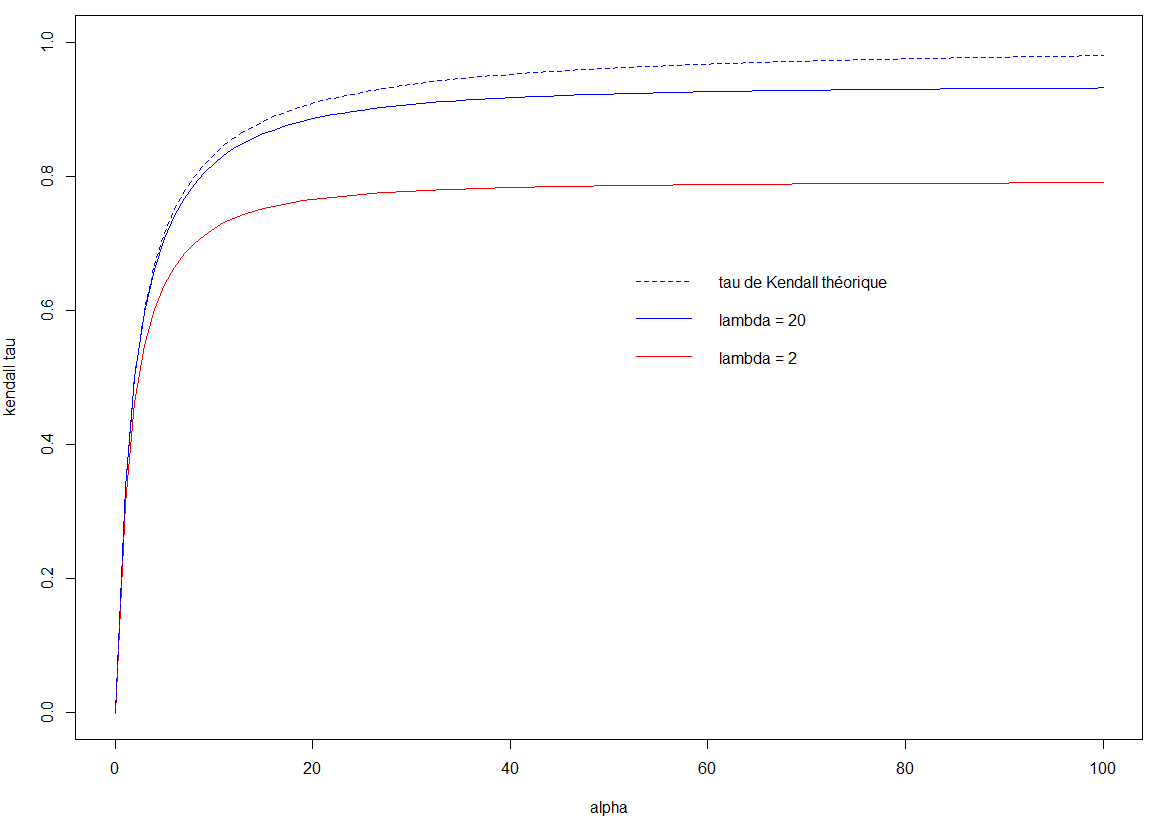
\includegraphics[height=6cm]{Graph/clayton.png}
	 	\caption[Copule de Clayton]{Graphique du tau de Kendall empirique selon la valeur du paramètre d'une copule de Clayton, pour un couple de variables aléatoires mixtes ou $N\sim Pois(\lambda)$, $\lambda = 2,20$ et $X \sim Exp(1/100)$. Le tau de Kendall empirique est calculé sur des échantillons de taille 10 000.} 
	 	\label{graph_clayton}
	 \end{figure}
 
 	Le même phénomène est illustré dans l'illustration \ref{graph_frank}. Une copule de Frank y est choisie afin d'observer le comportement du tau de Kendall dans le cas d'une dépendance négative. Comme précédemment plus le paramètre de la variable discrète augmente plus le tau de Kendall a une amplitude élevé. Alors, lorsque la variable aléatoire discrète possède un grand nombre de valeurs possibles son impact sur la valeur du tau de Kendall diminue.
	 
	 \begin{figure}[H]
	 	\centering
	 	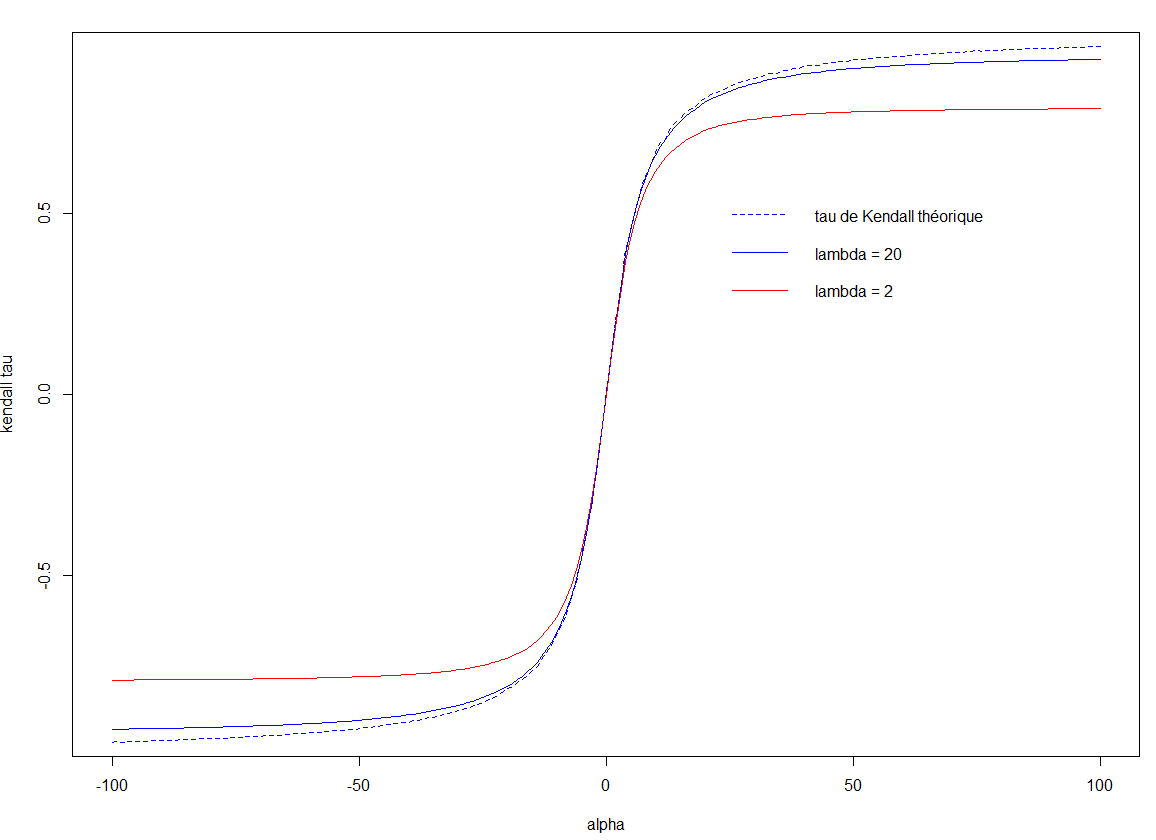
\includegraphics[height=6cm]{Graph/frank.png}
	 	\caption[Copule de Frank]{Graphique du tau de Kendall empirique selon la valeur du paramètre d'une copule de Frank, pour un couple de variables aléatoires mixtes ou $N\sim Pois(\lambda)$, $\lambda = 2,20$ et $X \sim Exp(1/100)$. Le tau de Kendall empirique est calculé sur des échantillons de taille 10 000.} 
	 	\label{graph_frank}
	 \end{figure}
	 
	 \subsection{Convergence asymptotique}
	 
	 L'illustration \ref{graph_asymptotique} représente le tau de Kendall théorique, lorsque les deux lois sont continues, et le tau de Kendall empirique, lorsqu'une des deux lois est discrète, selon le paramètre d'une copule de Clayton. Le tau de Kendall est calculé par \eqref{eq_tau_discret_empirique} avec des échantillons de taille 10\,000, pour un couple de variables aléatoires mixtes ou $N\sim Pois(50)$ et $X \sim Exp(1/100)$. Ainsi asymptotiquement le tau de Kendall empirique converge vers le tau de Kendall théorique lorsque le paramètre de la variable aléatoire discrète est assez grand.
	 
	 \begin{figure}[H]
	 	\centering
	 	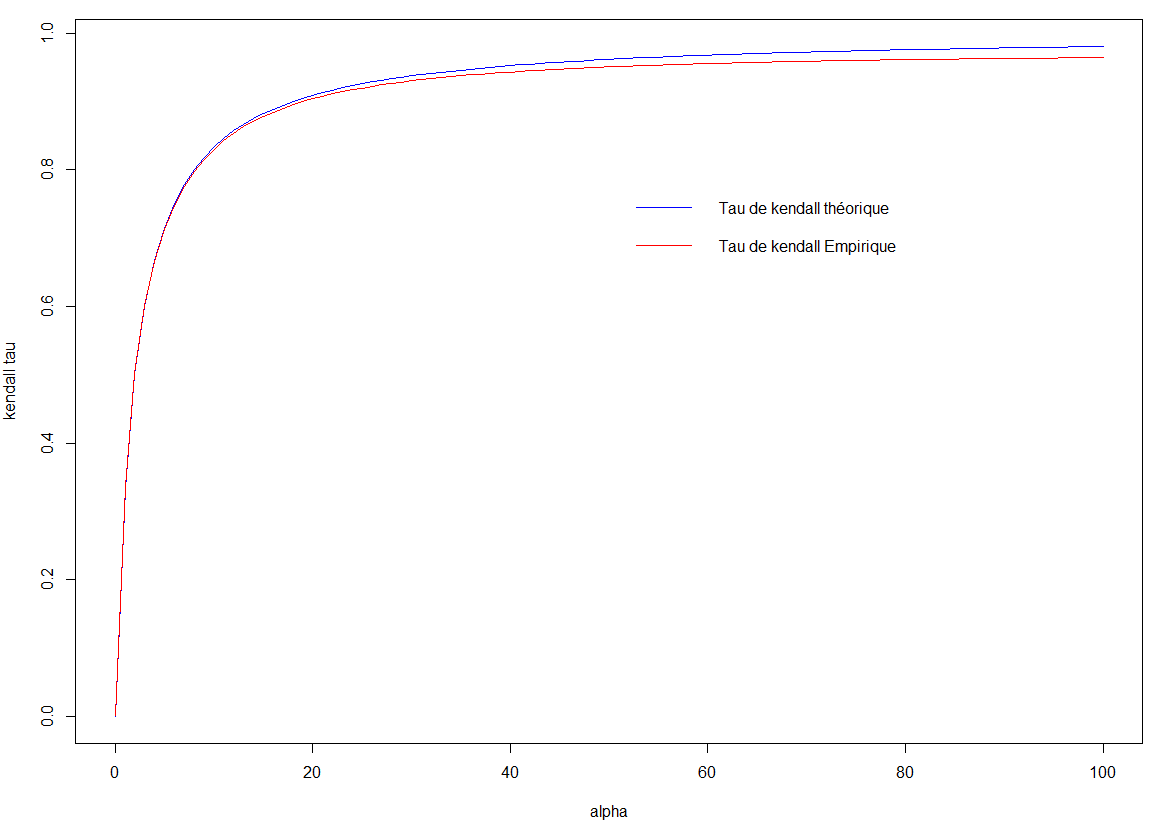
\includegraphics[height=6cm]{Graph/asymptotique.png}
	 	\caption[Comportement asymptotique]{Graphique du tau de Kendall théorique et empirique selon la valeur du paramètre d'une copule de Clayton. Le tau de kendall empirique est calculé pour un couple de variables aléatoires mixtes ou $N\sim Pois(50)$ et $X \sim Exp(1/100)$. Le tau de kendall théorique est obtenu par la formule $\alpha/(\alpha+2)$.} 
	 	\label{graph_asymptotique}
	 \end{figure}
 
 \newpage
 	\section{Calculs numériques}
 	
 	Lorsqu'on désire trouver le paramètre de dépendance par la méthode des moments (via le tau de Kendall ou le rho de Spearman), il faut d'abord être en mesure de calculer la valeur théorique des mesures de dépendance. À cet effet, le code informatique \ref{code_Kendall_theorique} permet de calculer le tau de Kendall théorique.
 	\begin{code}\label{code_Kendall_theorique}
 		\begin{verbatim}
 		
 		
		library(copula)
		library(rlist)
 		
 		
		tau_kendall_theorique <- function(F_N, F_X, para, Copule, alpha, n_max, x_max){
		
		    # Fonction qui permet de calculer le tau de kendall avec une  
		    # variable aléatoire discrète et une autre qui est continue.
		
		    F_N. <- function(n) {
		        # Paramétriser la fonction de répartition de N.
		        do.call(F_N, list.flatten(list(q = n, para$N)))
		    }
		    F_X. <- function(x) {
		        # Paramétriser la fonction de répartition de X.
		        do.call(F_X, list.flatten(list(q = x, para$X)))
		    }
		
		    f_N <- function(n) F_N.(n) - F_N.(n-1)
		
		    F_NX <- function(n, x) {
		        # Fonction de répartition conjointe de N et X.
		        f <- function(U) pCopula(U, Copule(alpha, use.indepC = "FALSE"))
		        return(f(c(F_N.(n), F_X.(x))))
		    }
		
		    f_NX <- function(n, x) {
		        # Fonction de densité conjointe de N et X.
		        eps <- .Machine$double.eps^0.25
		        f <- function(n,x) (F_NX(n, x + eps) - F_NX(n, x)) / eps
		        return(f(n, x) - f(n - 1, x))
		    }
		
		    return(
		        sum(sapply(0:n_max, function(n)
		            4 * integrate(
		                Vectorize(function(x)
		                    F_NX(n - 1, x) * f_NX(n, x)),
		                0, x_max,
		                subdivisions = 100L,
		                rel.tol = .Machine$double.eps ^ 0.25
		                )$value +
		                    f_N(n) ^ 2)) - 1
		    )
		}
 		\end{verbatim}
 	\end{code}
 	\clearpage
 	
 	Les arguments pris par cette fonction sont
 	\begin{itemize}
 		\item \texttt{F\_N}: La fonction de répartition de la variable discrète (ex: \texttt{ppois}, \texttt{pbinom}, etc.);
 		\item \texttt{F\_X}: La fonction de répartition de la variable continue (ex: \texttt{pexp}, \texttt{pgamma}, etc.);
 		\item \texttt{para}: La liste des arguments qui servent à \texttt{F\_N} et \texttt{F\_X}; \\
 			(ex: pour $N\sim Binom(5, 0.4)$ et $X\sim Exp(1/100)$, on aurait \\ 
 			\texttt{para = list(N = list(size = 5, prob = 0.4), X = list(beta = 1/100))})
		\item \texttt{Copule}: Une classe du module \texttt{Copula} (ex: \texttt{frankCopula}, \texttt{amhCopula}, etc.) 
			\footnote{https://www.rdocumentation.org/packages/copula/versions/0.999-19/topics/archmCopula-class}
		\item \texttt{alpha}: Paramètre de dépendance inhérent à la famille de copule utilisée;
		\item \texttt{n\_max} et \texttt{x\_max}: Les valeurs maximales que peuvent prendre les variables aléatoires $N$ et $X$. \\
			(ex: pour $N\sim Poisson(1)$ et $X\sim Exp(1/100)$, on aurait \\ 
			\texttt{n\_max = qpois(0.99999, 1); x\_max = qexp(0.99999, 1/100)})\\
 	\end{itemize}
 
 	Maintenant que l'on peut calculer la valeur théorique du tau de Kendall pour un couple de variables aléatoires mixtes, il est possible d'inverser la fonction numériquement afin d'identifier le paramètre de dépendance d'un jeu de données à l'aide de l'estimation trouvée avec le code informatique \ref{code_Kendall_empirique}. On y parvient avec le code informatique \ref{code_inversion_tau_kendall}.
 	
 	\begin{code}\label{code_inversion_tau_kendall}
 		\begin{verbatim}
 		
 		
 		inversion_tau_kendall <- function(F_N, F_X, para, Copule, bornes, tau, n_max, x_max){
 		
 		    # Fonction qui permet de trouver le paramètre de dépendance à l'aide du 
 		    # tau de Kendall empirique lorsque le modèle comprend une v.a. discrète et
 		    # une v.a. continue.

 		    alpha <- uniroot(function(alpha)
 		                tau_kendall_theorique(F_N, F_X, para, 
 		                    Copule, alpha, n_max, x_max) - tau,
 		            bornes)$root)
 		        
 		    return(alpha)
 		}
 		\end{verbatim}
 	\end{code}
 	%
	 Pour cette fonction, les paramètre sont les mêmes que dans le code informatique \ref{code_Kendall_theorique} à l'exception du paramètre \texttt{alpha} qui est remplacé par \texttt{tau}. Ce dernier représente le tau empirique que l'on désire inverser pour trouver le paramètre de dépendance de la copule. De plus, l'argument \texttt{bornes} est un vecteur représentant l'intervalle des valeurs possibles du paramètre de dépendance. Afin de réduire les temps de calcul et maximiser les chances de trouver une solution à l'optimisation numérique, le mieux est de faire une analyse graphique pour identifier l'intervalle le plus petit possible dans lequel on veut appliquer la fonction. Des exemples d'application de cette procédure sont présentés dans la sous-section \ref{subsect_exemples_inversion}
	 
	 \subsection{Exemples d'inversion du tau de Kendall}\label{subsect_exemples_inversion}
	 
	 Avec les formules proposées dans les codes informatiques \ref{code_Kendall_empirique}, \ref{code_Kendall_theorique} et \ref{code_inversion_tau_kendall}, on cherche à inverser un tau de Kendall calculé empiriquement sur une base de données afin d'identifier le paramètre qui façonne la structure de dépendance entre une variable aléatoire discrète et une qui est continue. Dans les exemples suivants, une méthodologie est proposée pour arriver à cette fin. Pour attester de la précision des codes informatiques définis dans la présente section, on utilise des données simulées dont on connaît le vrai paramètre de dépendance. \\
	 
	 \clearpage
	 \begin{scenario}
	 	\textbf{Copule de Frank}:
	 	\label{scenario_Frank}
	 \end{scenario}
 	 Posons un modèle de dépendance construit sur une copule de Frank, avec comme paramètre $\alpha = 5$, et dont les deux variables aléatoires qui le composent sont $N \sim Pois(1)$ et $X\sim Exp(1/100)$. 
 	 On pose les paramètre en \texttt{R} comme démontré dans le code informatique \ref{code_parametres}. \\
 	 
	 \begin{minipage}[H]{\linewidth}
 	 	\begin{code}\label{code_parametres}
	 	 \begin{verbatim}
	 	 
	 	 
		 	 alpha <- 5
		 	 Copule <- frankCopula
		 	 F_N <- ppois
		 	 F_X <- pexp
		 	 para <- list(N=list(lambda=2), X=list(rate=1/100))
		 	 n_max <- qpois(0.99999, para$N$lambda)
		 	 x_max <- qexp(0.99999, para$X$rate)
	 	 \end{verbatim}
	 	\end{code}
 	\end{minipage}

 	On estime un tau de Kendall empiriquement. Dans ce cas-ci, on simule 1\,000 réalisations du couple $(X_i, Y_i)$. Puis, pour obtenir un intervalle de confiance sur l'estimateur obtenu, on répète cette simulation 1\,000 fois. Comme il est illustré dans le code informatique \ref{code_simul}. Dans une situation où on aurait un vrai jeu de données, on pourrait avoir recours à la méthode du ré-échantillonnage (\textit{bootstrap}) afin de définir cet intervalle. \\

	 \begin{minipage}[H]{\linewidth}
 	 	 	\begin{code}\label{code_simul}
	 		\begin{verbatim}
	 		
	 		
				tau_empirique <- numeric(nsim <- 1e+3)
				set.seed(20190618)
				for (i in 1:nsim) {
				    UU <- rCopula(1e+3, Copule(alpha))
				    X <- qpois(UU[,1], para$N$lambda)
				    Y <- qexp(UU[,2], para$X$rate)
				    tau_empirique[i] <- tau_kendall_empirique(X, Y)
				}
				mean_tau <- mean(tau_empirique)
	 		\end{verbatim}
 			\end{code}
 	\end{minipage}

 	Dans le contexte du scénario \ref{scenario_Frank}, on obtient, pour un niveau de confiance de 95\%, que $\tau_n \in [0.4007240, 0.4594975]$ et la moyenne est de $0.4301108$. Avec le code informatique \ref{code_Kendall_theorique}, on trouve que $\tau = 0.4299595$; ce qui signifie que l'estimateur empirique est sans biais puisqu'il appartient à cet intervalle. À cet effet, dans l'illustration \ref{graph_Tau_n_asymptotique}, on voit que le comportement asymptotique de l'estimateur $\tau_n$ obéit à une loi normale.
 	
 		\begin{figure}[H]
 		\centering
 		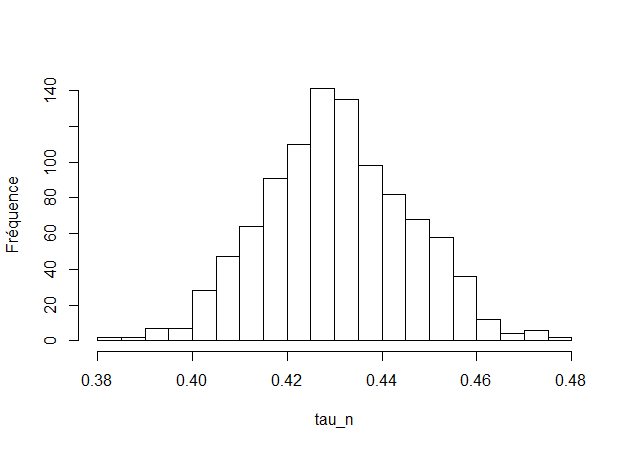
\includegraphics[height=8cm]{Graph/Tau_n_asymptotique.png}
 		\caption{Comportement asymptotique de $\tau_n$ avec 1\,000 simulations.} 
 		\label{graph_Tau_n_asymptotique}
 	\end{figure}
 	
 	
 	Maintenant, afin de trouver le paramètre de dépendance du jeu de données simulé, il faut identifier l'intervalle optimal sur lequel appliquer la fonction présentée dans le code informatique \ref{code_inversion_tau_kendall}. Le code \ref{code_graphique_intervalle} permet donc de générer l'illustration \ref{graph_intervalle_Frank}. \\
 	
	 \begin{minipage}[H]{\linewidth}
 	 	 	\begin{code} \label{code_graphique_intervalle}
	 		\begin{verbatim}
	 		
	 		
	 		Tau <- sapply(c(-5:-1, 1:10), function(a)
	 		    tau_kendall_theorique(F_N, F_X, para, Copule, a, n_max, x_max))
	 		
	 		plot(c(-5:-1, 1:10), Tau,
	 		    ylab="tau de kendall",
	 		    xlab="alpha",
	 		    type="l"
	 		)
	 		axis(2, tck = 1, lty = 2, col = "grey") # L'axe des ordonnées
	 		axis(1,at=-5:10, tck=1, lty = 2, col = "grey",) # L'axe des abscisses
	 		abline(a=tau_empirique, b=0, col="green")
	 		\end{verbatim}
 			\end{code}
 	\end{minipage}

	\begin{figure}[H]
		\centering
		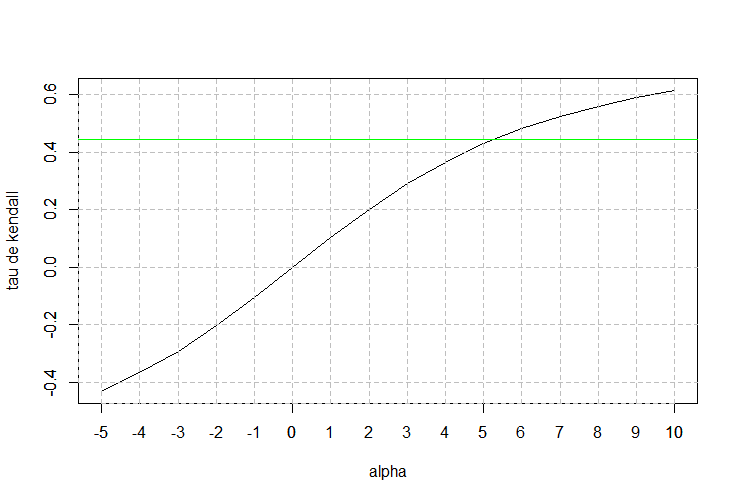
\includegraphics[height=8cm]{Graph/intevalle_frank.png}
		\caption[Identification de l'intervalle d'optimisation numérique pour le scénario \ref{scenario_Frank}]
		{Identification de l'intervalle d'optimisation numérique pour une copule de Frank avec $\alpha = 5$.} 
		\label{graph_intervalle_Frank}
	\end{figure}

	Avec l'illustration \ref{graph_intervalle_Frank}, on voit qu'un intervalle optimal pourrait être $[4.5, 5.5]$. Il ne reste donc plus qu'à utiliser le code \ref{code_inversion_tau_kendall} pour obtenir les résultats présentés dans le tableau \ref{tbl_Resultats_Frank}.
	
	\begin{table}[H]
		\centering
		\begin{tabular}{lr}
			\hline
			Vrai paramètre & 5.0000 \\ 
			Paramètre trouvé & 5.0026 \\ 
			Temps d'optimisation & 9.7800 \\ 
			\hline
		\end{tabular}
	\caption{Résultats de l'inversion du tau de Kendall avec une copule de Frank.}
	\label{tbl_Resultats_Frank}
	\end{table}

	Dans le tableau \ref{tbl_Resultats_Frank}, on voit que le paramètre trouvé est très proche de la vraie valeur de $\alpha$. 
	
 	
 	\begin{scenario}
 		\textbf{Copule de AMH}:
 		\label{scenario_AMH}
 	\end{scenario}
 	 Posons un modèle de dépendance construit sur une copule de AMH, avec comme paramètre $\alpha = 0.5$, et dont les deux variables aléatoires demeurent inchangées par rapport au scénario \ref{scenario_Frank}. 
 	 L'attribution des paramètres se fait de façon similaire à celle présentée dans le code informatique \ref{code_parametres}. En gardant le même encrage de simulation (\textit{seed}), on obtient que $\tau_n \in [0.08199922, 0.16145825]$ et la moyenne est de $0.1217287$, pour un $\tau$ théorique de $0.1220402$. Par la suite, par analyse graphique, on voit dans l'illustration \ref{graph_intervalle_AMH} que $\alpha \in [0.45, 0.55]$. Par inversion du tau empirique moyen, on obtient le tableau \ref{tbl_Resultats_AMH} qui présente les résultats de la simulation.\\
 	 
 	 \begin{figure}[H]
 	 	\centering
 	 	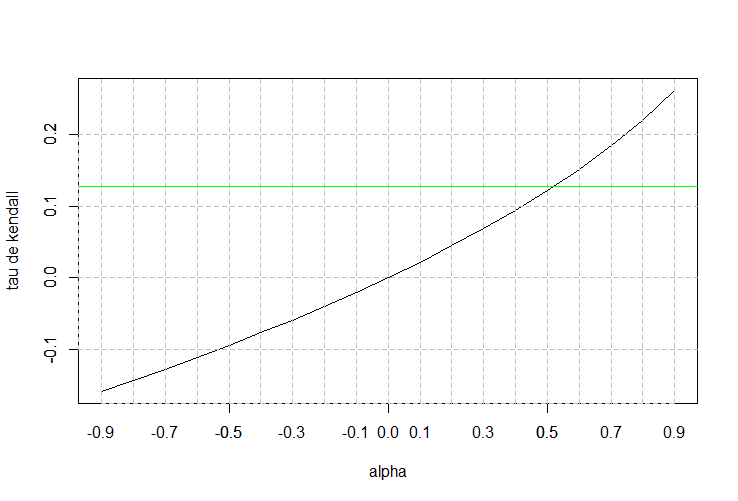
\includegraphics[height=8cm]{Graph/intevalle_AMH.png}
 	 	\caption[Identification de l'intervalle d'optimisation numérique pour le scénario \ref{scenario_AMH}]
 	 	{Identification de l'intervalle d'optimisation numérique pour une copule de AMH avec $\alpha = 0.5$.} 
 	 	\label{graph_intervalle_AMH}
 	 \end{figure}
  
  	 \begin{table}[H]
  		\centering
  		\begin{tabular}{lr}
  			\hline
  			Vrai paramètre & 0.5000 \\ 
  			Paramètre trouvé & 0.4989 \\ 
  			Temps d'optimisation & 6.6100 \\
  			\hline 
  		\end{tabular}
  		\caption{Résultats de l'inversion du tau de Kendall avec une copule de AMH.}
  		\label{tbl_Resultats_AMH}
  	\end{table}
  
  	Comme pour le scénario \ref{scenario_Frank}, on observe un bon niveau de précision.
  	
 	 
 	\begin{scenario}
 		\textbf{Copule de Gumbel}:
 		\label{scenario_Gumbel}
 	\end{scenario}
	Posons un modèle de dépendance construit sur une copule de Gumbel, avec comme paramètre $\alpha = 5$, et dont les deux variables aléatoires demeurent inchangées par rapport aux scénarios \ref{scenario_Frank} et \ref{scenario_AMH}. Toujours avec le même encrage de simulation, on a $\tau_n \in [0.7028951, 0.7350736]$ et une moyenne de $0.7189843$ pour un $\tau$ théorique de $0.7194499$. Avec l'aide de l'illustration \ref{graph_intervalle_Gumbel}, on voit que $\alpha \in [4.5, 5.5]$. On obtient alors les résultats présentés dans le tableau \ref{tbl_Resultats_Gumbel}.
	
	\begin{figure}[H]
		\centering
		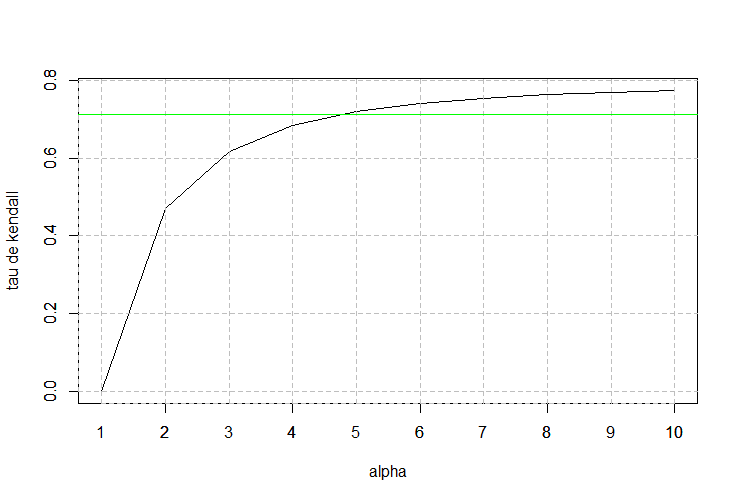
\includegraphics[height=8cm]{Graph/intevalle_Gumbel.png}
		\caption[Identification de l'intervalle d'optimisation numérique pour le scénario \ref{scenario_Gumbel}]
		{Identification de l'intervalle d'optimisation numérique pour une copule de Gumbel avec $\alpha = 5$.} 
		\label{graph_intervalle_Gumbel}
	\end{figure}
	
	\begin{table}[H]
		\centering
		\begin{tabular}{lr}
			\hline
			Vrai paramètre & 5.0000 \\ 
			Paramètre trouvé & 4.9827 \\ 
			Temps d'optimisation & 21.5200 \\ 
			\hline 
		\end{tabular}
		\caption{Résultats de l'inversion du tau de Kendall avec une copule de Gumbel.}
		\label{tbl_Resultats_Gumbel}
	\end{table}


	\begin{scenario}
		\textbf{Copule de Joe}:
		\label{scenario_Joe}
	\end{scenario}
	Finalement, si on pose un modèle de dépendance construit sur une copule de Joe, avec comme paramètre $\alpha = 5$, et dont les autres hypothèses restent inchangées. On a $\tau_n \in [0.6008445, 0.6502252]$ et une moyenne de $0.6255349$ pour un $\tau$ théorique de $0.6260815$. Avec l'aide de l'illustration \ref{graph_intervalle_Joe}, on voit que $\alpha \in [4.5, 6.5]$. On obtient alors les résultats présentés dans le tableau \ref{tbl_Resultats_Joe}.
	
	\begin{figure}[H]
		\centering
		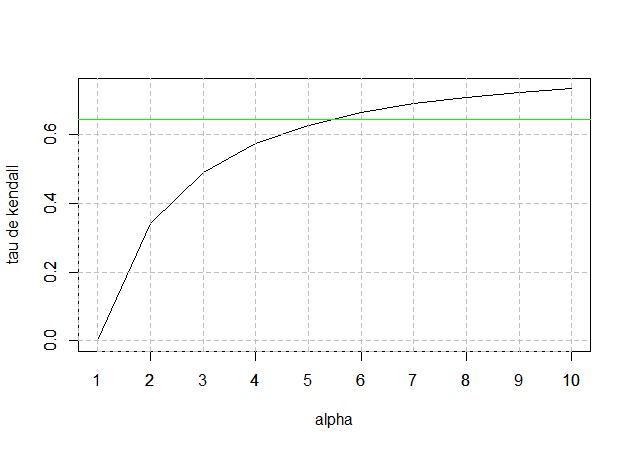
\includegraphics[height=8cm]{Graph/intevalle_Joe.png}
		\caption[Identification de l'intervalle d'optimisation numérique pour le scénario \ref{scenario_Joe}]
		{Identification de l'intervalle d'optimisation numérique pour une copule de Joe avec $\alpha = 5$.} 
		\label{graph_intervalle_Joe}
	\end{figure}
	
	\begin{table}[H]
		\centering
		\begin{tabular}{lr}
			\hline
			Vrai paramètre & 5.0000 \\ 
			Paramètre trouvé & 4.9827 \\ 
			Temps d'optimisation & 21.5200 \\ 
			\hline 
		\end{tabular}
		\caption{Résultats de l'inversion du tau de Kendall avec une copule de Joe.}
		\label{tbl_Resultats_Joe}
	\end{table}

	
	\section{Modèle collectif du risque}
	\subsection{Estimation de $\alpha_{0}$}
	
	Dans cette section la méthode d'estimation précédente est appliquée au modèle collectif du risque avec $N \sim Binom(7,0.4) $ et $X \sim Exp(1/100)$. Les exemples suivants illustrent les cas où la loi mère est logarithmique ou géométrique et la loi enfant est gamma. Les estimations ont été réalisées avec des simulations d'échantillons de taille 10 000. Trois estimateurs de $\alpha_{0}$ sont calculés selon la méthode de calcul du tau de Kendall empirique, le premier utilise le tau de Kendall entre $N$ et $X_{1}$, le second la moyenne des taus de Kendall entre $N$ et $X_{i},i=1,2,3,4$ et le dernier la moyenne des taus de Kendall entre $N$ et tous les $X_{i}$. On ne prends pas en compte les valeurs où $N$ est nul. Pour les $X_{i}$ le tau de Kendall est calculé lorsque $X_{i}$ est défini.
	
	\begin{scenario}
		\textbf{Copule hiérarchique Logarithmique-Gamma de paramètres $(\alpha_{0}=5,\alpha_{1}=4)$}:
		\label{scenario_log-gamma}
	\end{scenario}
	
	Dans ce cas la copule utilisée est la copule de Frank de paramètre $\alpha_{0}$. Le tableau \ref{MCR_Frank} illustrent le résultat de l'estimation :
	
	\begin{table}[ht]
		\centering
		\begin{tabular}{rrrrr}
			\hline
			& Paramètre & Estimateur 1 & Estimateur 2 & Estimateur 3 \\ 
			\hline
			& 5.0000 & 5.0744 & 3.7114 & 1.9643 \\
			\hline
		\end{tabular}
		\caption{Tableau présentant les estimateurs de $\alpha_{0}$. L'estimateur 1 prend le tau de Kendall entre $N$ et $X_{1}$, l'estimateur 2 la moyenne des taus de Kendall entre $N$ et $X_{i},i=1,2,3,4$, l'estimateur 3 la moyenne des taus de Kendall entre $N$ et tous les $X_{i}$. }
		\label{MCR_Frank}
	\end{table}
	
	\begin{scenario}
		\textbf{Copule hiérarchique Géométrique-Gamma de paramètres $(\alpha_{0}=0.6,\alpha_{1}=4)$}:
		\label{scenario_geo-gamma}
	\end{scenario}
	
	Dans ce cas la copule utilisée est la copule AMH de paramètre $\alpha_{0}$. Le tableau \ref{MCR_AMH} illustre le résultat de l'estimation :
	
	\begin{table}[ht]
		\centering
		\begin{tabular}{rrrrr}
			\hline
			& Paramètre & Estimateur 1 & Estimateur 2 & Estimateur 3 \\ 
			\hline
			& 0.6000 & 0.6166 & 0.4367 &  0.2963 \\
			\hline
		\end{tabular}
		\caption{Tableau présentant les estimateurs de $\alpha_{0}$. L'estimateur 1 prend le tau de Kendall entre $N$ et $X_{1}$, l'estimateur 2 la moyenne des taus de Kendall entre $N$ et $X_{i},i=1,2,3,4$, l'estimateur 3 la moyenne des taus de Kendall entre $N$ et tous les $X_{i}$. }
		\label{MCR_AMH}
	\end{table}
	
	Le fait de prendre en compte les taus de Kendall entre $N$ et tous les $X_{i}$ n'améliore pas la qualité de l'estimation. La meilleure option reste de prendre le tau de Kendall entre $N$ et $X_{1}$.

	\subsection{Estimation de $\alpha_{1}$}
	
	Le modèle collectif du risque est modélisé par une copule hiérarchique à deux paramètres. Le premier paramètre $\alpha_{0}$, paramètre de la loi mère modélise la dépendance entre $N$ et $X$, il a été estimé dans la section précédente. Le second paramètre $\alpha_{1}$, paramètre de la loi enfant modélise la dépendance entre les $X_{i}$. Étant donné que les $X_{i}$ sont des variables continues pour calculer le tau de Kendall empirique entre $X_{i}$ et $X_{j}$ on utilise la formule suivante :
	
	\begin{equation}\label{eq_tau_continu}
	\tau (X_{i},X_{j}) = 4 \int_{0}^{1}\int_{0}^{1} C(u_{1},u_{2})c(u_{1},u_{2}) - 1.
	\end{equation}
	où  \[ C(u_{1},u_{2}) = \mathscr{L}_{\Theta}(\mathscr{L}_{\Theta}^{-1}(u_{1}) + \mathscr{L}_{\Theta}^{-1}(u_{2}) )  \]
	avec    \[ \mathscr{L}_{\Theta}(t) = \mathscr{L}_{M}(-\ln(\mathscr{L}_{B}(t))) \]
	et	\[ c(u_{1},u_{2}) =  \frac{\partial^2}{\partial u_{1}\partial u_{2}}C(u_{1},u_{2})  \]
	
	La relation entre les $X_{i}$ est modélisée par une copule archimédienne à deux paramètres, il faut donc pour l'estimation de $\alpha_{1}$ estimer préalablement $\alpha_{0}$. 
	Les tableaux \ref{resultats_alpha1} et \ref{resultats_alpha1tous} présentent les résultats de l'estimation de $\alpha_{1}$, le paramètre $\alpha_{0}$ utilisé pour l'estimation et le temps d'estimation comprenant l'estimation des deux paramètres de la copule archimédienne hiérarchique. Le tau de Kendall empirique entre les variables continues et la variable discrète est calculé à partir des variables $N$ et $X_{1}$. Pour le tableau \ref{resultats_alpha1} le tau de Kendall entre les variables continues est calculé par les variables $X_{1}$ et $X_{2}$. Pour le tableau \ref{resultats_alpha1tous} le tau de Kendall empirique entre les variables continues est la moyenne des taus de Kendall entre tous les $X_{i}$.L'ajout des taus de Kendall entre toutes les variables détériore la qualité de l'estimation en raison du manque d’informations. Afin de pouvoir comparer ces deux résultats, les estimations par les deux méthodes sont effectuées à partir des mêmes échantillons.
	
	\begin{table}[H]
		\centering
		\begin{tabular}{rrrrr}
			\hline
			& Paramètre $\alpha_{0}$ & Estimateur $\alpha_{0}$ & Paramètre $\alpha_{1}$ & Estimateur $\alpha_{1}$  \\ 
			\hline
			Géométrique-Géométrique & 0.6000 & 0.6064 & 0.4000 & 0.4375  \\ 
			Géométrique-Logarithmique & 0.6000 & 0.6037 & 7.0000 & 6.7736 \\ 
			Géométrique-Gamma & 0.6000 & 0.6212 & 4.0000 & 3.8284 \\ 
			Logarithmique-Logarithmique & 4.0000 & 3.9243 & 7.0000 & 5.8620  \\ 
			Logarithmique-Géométrique & 5.0000 & 5.0307 & 0.6000 & 0.2811 \\ 
			Logarithmique-Gamma & 6.0000 & 5.7881 & 4.0000 & 2.5337  \\  
			\hline
		\end{tabular}
		\begin{tabular}{rr}
			\hline
			& Temps \\ 
			\hline
			Géométrique-Géométrique & 37.5900 \\ 
			Géométrique-Logarithmique  & 38.9700 \\ 
			Géométrique-Gamma & 36.5300 \\ 
			Logarithmique-Logarithmique & 66.8100 \\ 
			Logarithmique-Géométrique  & 63.2700 \\ 
			Logarithmique-Gamma  & 73.3800 \\  
			\hline
		\end{tabular}
		\caption{Tableau présentant les estimateurs de $\alpha_{1}$, les valeurs estimées de $\alpha_{0}$ utilisées ainsi que le temps de calcul. Le tau de Kendall empirique utilisé est le tau de Kendall entre $X_{1}$ et $X_{2}$. Les données utilisées sont issues de simulations d’échantillons de taille 10 000.}
		\label{resultats_alpha1}
	\end{table}
	
	
	\begin{table}[H]
		\centering
		\begin{tabular}{rrrrr}
			\hline
			& Paramètre $\alpha_{0}$ & Estimateur $\alpha_{0}$ & Paramètre $\alpha_{1}$ & Estimateur $\alpha_{1}$  \\  
			\hline
			Géométrique-Géométrique & 0.6000 & 0.6064 & 0.4000 & 0.3246 \\ 
			Géométrique-Logarithmique & 0.6000 & 0.6037 & 7.0000 & 6.1878 \\ 
			Géométrique-Gamma & 0.6000 & 0.6212 & 4.0000 & 2.7547  \\ 
			Logarithmique-Logarithmique & 4.0000 & 3.9243 & 7.0000 & 1.0010  \\ 
			Logarithmique-Géométrique & 5.0000 & 5.0307 & 0.6000 & 0.0001 \\ 
			Logarithmique-Gamma & 6.0000 & 5.7881 & 4.0000 & 0.4699 \\ 
			\hline
		\end{tabular}
		%
		\begin{tabular}{rr}
			\hline
			 & Temps \\  
			\hline
			Géométrique-Géométrique & 41.0400 \\ 
			Géométrique-Logarithmique & 42.1500 \\ 
			Géométrique-Gamma & 39.6800 \\ 
			Logarithmique-Logarithmique  & 69.7800 \\ 
			Logarithmique-Géométrique  & 66.6300 \\ 
			Logarithmique-Gamma  & 76.6200 \\ 
			\hline
		\end{tabular}
		\caption{Tableau présentant les estimateurs de $\alpha_{1}$, les valeurs estimées de $\alpha_{0}$ utilisées ainsi que le temps de calcul. Le tau de Kendall empirique utilisé la moyenne de tous les taus de Kendall. Les données utilisées sont issues de simulation d’échantillons de taille 10 000.}
		\label{resultats_alpha1tous}
	\end{table}

	\section{Conclusion}
	Dans la littérature le tau de Kendall est calculé pour des variables aléatoires continues ou des variables aléatoires discrètes. Le lemme \ref{eq_tau} propose une formule qui permet de calculer le tau de Kendall dans le cas ou une des variables est discrète et l'autre est continue.
	Dans le cas des variables aléatoires discrètes, le choix des lois a un impact sur le tau de Kendall a cause des observations qui se répètent. Ainsi plus le nombre de valeurs prises par la variable aléatoire discrète est grand plus ce phénomène s'atténue.
	Le lemme \ref{lemme} et le lemme \ref{lemme_empirique} nous permettent de réaliser une optimisation numérique afin de déterminer le paramètre $\alpha_0$ des copules archimédiennes hiérarchiques utilisées dans le modèle collectif du risque. 
	De la même façons la formule \ref{eq_tau_continu} nous permet d'obtenir le paramètre $\alpha_{1}$ de la copule archimédienne hiérarchique. Pour le modèle collectif du risque prendre un grand nombre de $X_i$ pour le calcul du tau de Kendall empirique n'améliore pas l'estimation des paramètres $\alpha_0$ et $\alpha_1$.


	\newpage
	\bibliography{BibRRT_Kendall.bib}
	\bibliographystyle{apalike}
	 
	 
\end{document}